\begin{frame}{Экспериментальные результаты}
\centering
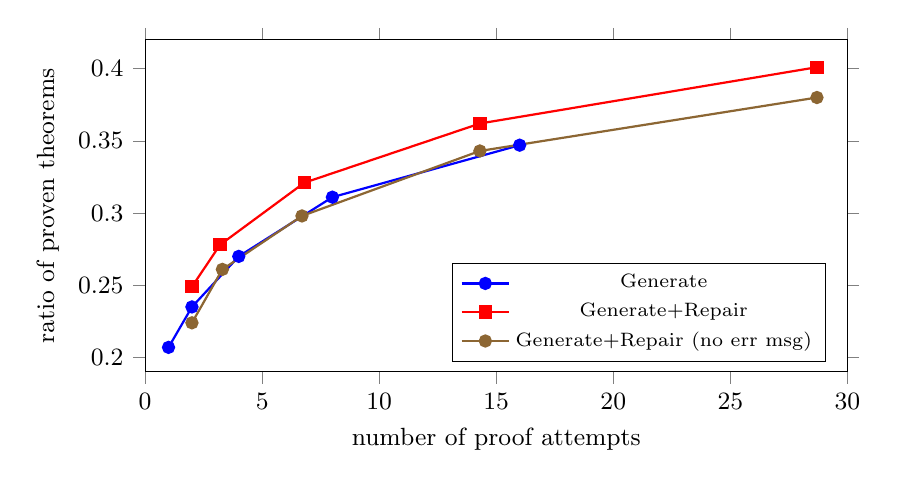
\begin{tikzpicture}
\begin{axis}[
    width=10.5cm,
    height=5.8cm,
    xmin=0, xmax=30,
    ymin=0.19, ymax=0.42,
    xlabel={number of proof attempts},
    ylabel={ratio of proven theorems},
    xtick={0,5,10,15,20,25,30},
    ytick={0.20,0.25,0.30,0.35,0.40},
    legend style={
        at={(0.97,0.03)},
        anchor=south east,
        draw=black,
        fill=white,
        font=\scriptsize
    },
    label style={font=\small},
    tick label style={font=\small},
    tick align=outside,
]

\addplot[color=blue, mark=*, thick] coordinates {
    (1,0.207)
    (2,0.235)
    (4,0.270)
    (8,0.311)
    (16,0.347)
};
\addlegendentry{Generate}

\addplot[color=red, mark=square*, thick] coordinates {
    (2,0.249)
    (3.2,0.278)
    (6.8,0.321)
    (14.3,0.362)
    (28.7,0.401)
};
\addlegendentry{Generate+Repair}

\addplot[color={rgb,1:red,0.55;green,0.40;blue,0.20}, mark=*, thick] coordinates {
    (2,0.224)
    (3.3,0.261)
    (6.7,0.298)
    (14.3,0.343)
    (28.7,0.380)
};
\addlegendentry{Generate+Repair (no err msg)}

\end{axis}
\end{tikzpicture}

\vspace{0.2cm}
{\small Ratio of theorems proven vs inference cost}
\end{frame}